% Options for packages loaded elsewhere
% Options for packages loaded elsewhere
\PassOptionsToPackage{unicode}{hyperref}
\PassOptionsToPackage{hyphens}{url}
\PassOptionsToPackage{dvipsnames,svgnames,x11names}{xcolor}
%
\documentclass[
  letterpaper,
  DIV=11,
  numbers=noendperiod]{scrartcl}
\usepackage{xcolor}
\usepackage{amsmath,amssymb}
\setcounter{secnumdepth}{-\maxdimen} % remove section numbering
\usepackage{iftex}
\ifPDFTeX
  \usepackage[T1]{fontenc}
  \usepackage[utf8]{inputenc}
  \usepackage{textcomp} % provide euro and other symbols
\else % if luatex or xetex
  \usepackage{unicode-math} % this also loads fontspec
  \defaultfontfeatures{Scale=MatchLowercase}
  \defaultfontfeatures[\rmfamily]{Ligatures=TeX,Scale=1}
\fi
\usepackage{lmodern}
\ifPDFTeX\else
  % xetex/luatex font selection
\fi
% Use upquote if available, for straight quotes in verbatim environments
\IfFileExists{upquote.sty}{\usepackage{upquote}}{}
\IfFileExists{microtype.sty}{% use microtype if available
  \usepackage[]{microtype}
  \UseMicrotypeSet[protrusion]{basicmath} % disable protrusion for tt fonts
}{}
\makeatletter
\@ifundefined{KOMAClassName}{% if non-KOMA class
  \IfFileExists{parskip.sty}{%
    \usepackage{parskip}
  }{% else
    \setlength{\parindent}{0pt}
    \setlength{\parskip}{6pt plus 2pt minus 1pt}}
}{% if KOMA class
  \KOMAoptions{parskip=half}}
\makeatother
% Make \paragraph and \subparagraph free-standing
\makeatletter
\ifx\paragraph\undefined\else
  \let\oldparagraph\paragraph
  \renewcommand{\paragraph}{
    \@ifstar
      \xxxParagraphStar
      \xxxParagraphNoStar
  }
  \newcommand{\xxxParagraphStar}[1]{\oldparagraph*{#1}\mbox{}}
  \newcommand{\xxxParagraphNoStar}[1]{\oldparagraph{#1}\mbox{}}
\fi
\ifx\subparagraph\undefined\else
  \let\oldsubparagraph\subparagraph
  \renewcommand{\subparagraph}{
    \@ifstar
      \xxxSubParagraphStar
      \xxxSubParagraphNoStar
  }
  \newcommand{\xxxSubParagraphStar}[1]{\oldsubparagraph*{#1}\mbox{}}
  \newcommand{\xxxSubParagraphNoStar}[1]{\oldsubparagraph{#1}\mbox{}}
\fi
\makeatother


\usepackage{longtable,booktabs,array}
\usepackage{calc} % for calculating minipage widths
% Correct order of tables after \paragraph or \subparagraph
\usepackage{etoolbox}
\makeatletter
\patchcmd\longtable{\par}{\if@noskipsec\mbox{}\fi\par}{}{}
\makeatother
% Allow footnotes in longtable head/foot
\IfFileExists{footnotehyper.sty}{\usepackage{footnotehyper}}{\usepackage{footnote}}
\makesavenoteenv{longtable}
\usepackage{graphicx}
\makeatletter
\newsavebox\pandoc@box
\newcommand*\pandocbounded[1]{% scales image to fit in text height/width
  \sbox\pandoc@box{#1}%
  \Gscale@div\@tempa{\textheight}{\dimexpr\ht\pandoc@box+\dp\pandoc@box\relax}%
  \Gscale@div\@tempb{\linewidth}{\wd\pandoc@box}%
  \ifdim\@tempb\p@<\@tempa\p@\let\@tempa\@tempb\fi% select the smaller of both
  \ifdim\@tempa\p@<\p@\scalebox{\@tempa}{\usebox\pandoc@box}%
  \else\usebox{\pandoc@box}%
  \fi%
}
% Set default figure placement to htbp
\def\fps@figure{htbp}
\makeatother

\ifLuaTeX
  \usepackage{luacolor}
  \usepackage[soul]{lua-ul}
\else
  \usepackage{soul}
\fi




\setlength{\emergencystretch}{3em} % prevent overfull lines

\providecommand{\tightlist}{%
  \setlength{\itemsep}{0pt}\setlength{\parskip}{0pt}}



 


\KOMAoption{captions}{tableheading}
\makeatletter
\@ifpackageloaded{caption}{}{\usepackage{caption}}
\AtBeginDocument{%
\ifdefined\contentsname
  \renewcommand*\contentsname{Table of contents}
\else
  \newcommand\contentsname{Table of contents}
\fi
\ifdefined\listfigurename
  \renewcommand*\listfigurename{List of Figures}
\else
  \newcommand\listfigurename{List of Figures}
\fi
\ifdefined\listtablename
  \renewcommand*\listtablename{List of Tables}
\else
  \newcommand\listtablename{List of Tables}
\fi
\ifdefined\figurename
  \renewcommand*\figurename{Figure}
\else
  \newcommand\figurename{Figure}
\fi
\ifdefined\tablename
  \renewcommand*\tablename{Table}
\else
  \newcommand\tablename{Table}
\fi
}
\@ifpackageloaded{float}{}{\usepackage{float}}
\floatstyle{ruled}
\@ifundefined{c@chapter}{\newfloat{codelisting}{h}{lop}}{\newfloat{codelisting}{h}{lop}[chapter]}
\floatname{codelisting}{Listing}
\newcommand*\listoflistings{\listof{codelisting}{List of Listings}}
\makeatother
\makeatletter
\makeatother
\makeatletter
\@ifpackageloaded{caption}{}{\usepackage{caption}}
\@ifpackageloaded{subcaption}{}{\usepackage{subcaption}}
\makeatother
\usepackage{bookmark}
\IfFileExists{xurl.sty}{\usepackage{xurl}}{} % add URL line breaks if available
\urlstyle{same}
\hypersetup{
  colorlinks=true,
  linkcolor={blue},
  filecolor={Maroon},
  citecolor={Blue},
  urlcolor={Blue},
  pdfcreator={LaTeX via pandoc}}


\author{}
\date{}
\begin{document}


\section{Predicting food web dynamics \&
diversity}\label{predicting-food-web-dynamics-diversity}

\begin{figure}[H]

{\centering 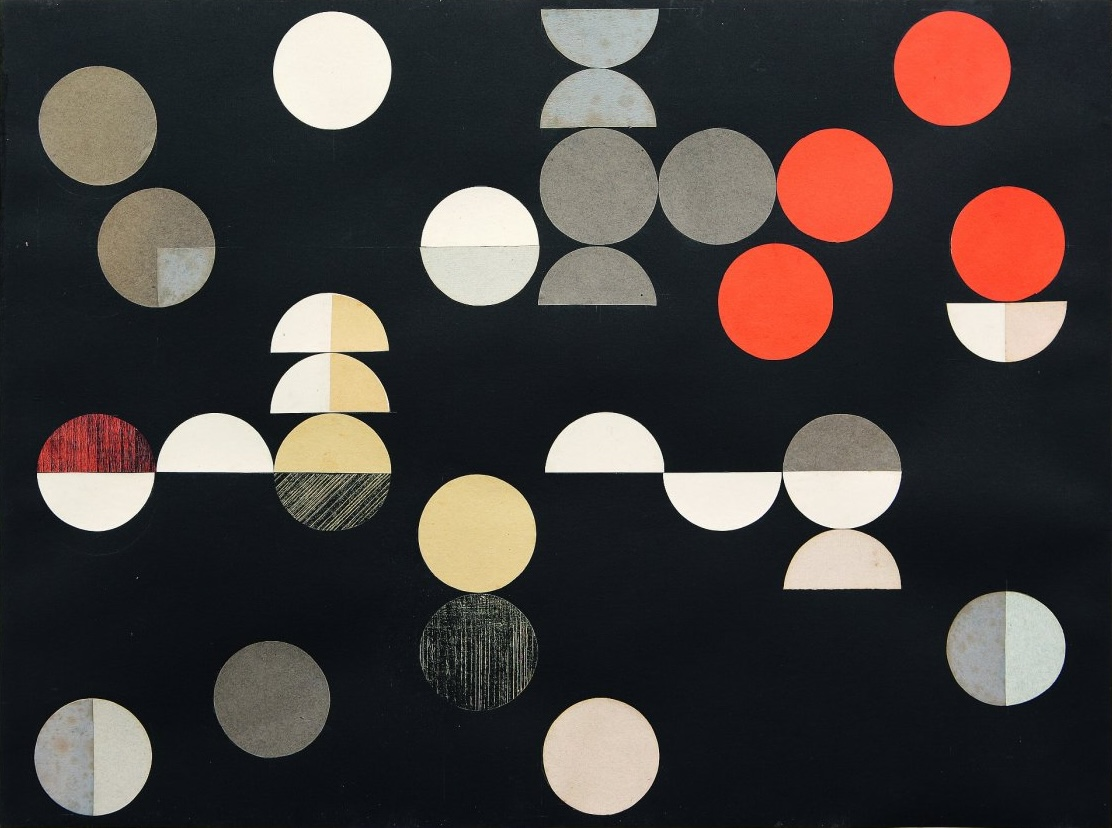
\includegraphics[width=8in,height=\textheight,keepaspectratio]{../static/arp-composition-with-circles-semicircles-1938.jpeg}

}

\caption{\emph{Composition with circles and semi-circles}, Sophie
Taeuber-Arp (1938)}

\end{figure}%

Predicting the coexistence of two species in a simple Lotka-Volterra
model has a tidy closed-form solution that is commonly taught in
undergraduate ecology classes. But add a third species, and solving the
problem suddenly becomes extremely difficult. Recent advances in
coexistence theory have offered a path forward, and our research is
confronting these approaches with empirical data.

\subsubsection{Community assembly \& coexistence in pitcher plant
microbes}\label{community-assembly-coexistence-in-pitcher-plant-microbes}

Communities can take dozens to hundreds of generations for competitive
exclusion to play out, greatly challenging our ability to test the
predictions of theory with typical ``fast'' cycling macroscopic
organisms like annual plants. The microbial communities of pitcher
plants (\emph{Sarracenia purpurea}) have generation times of several
hours and highly specialized associations with their host plant. We are
using this model system for lab and field experiments to probe the
mechanisms of multispecies community assembly and coexistence.
Furthermore, Ph.D.~student \href{../people/burroughs-n/about.qmd}{Nicole
Burroughs} is examining the repeatability of community assembly and
testing how variation in microbial dispersal determines the likelihood
of alternative assembly pathways.

\begin{figure}[H]

{\centering 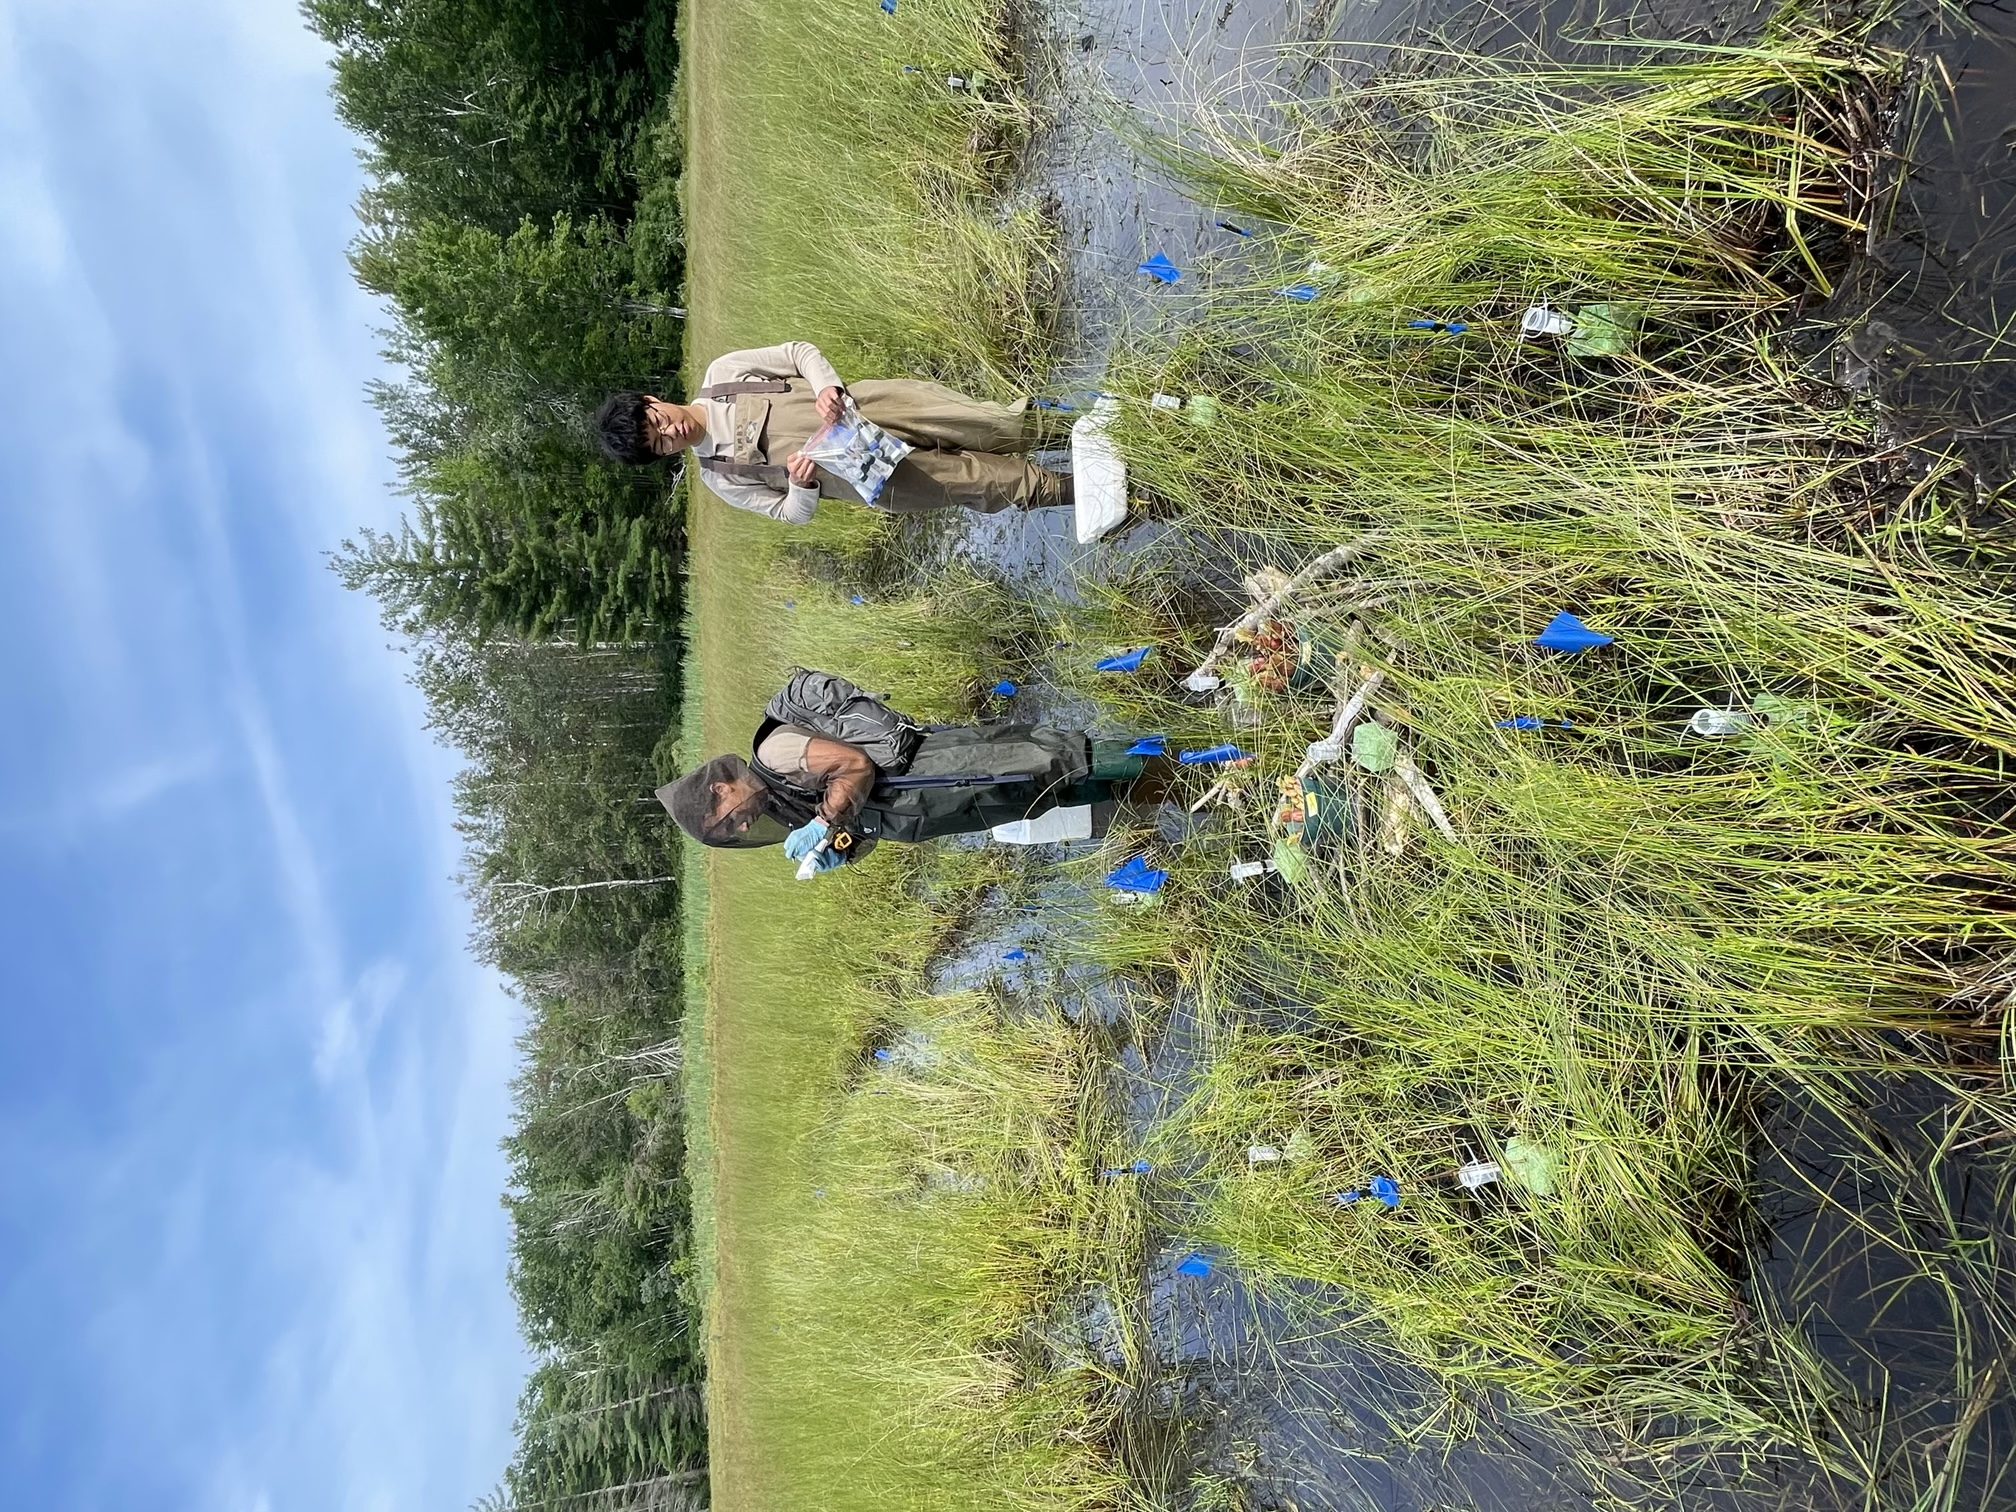
\includegraphics[width=4.5in,height=\textheight,keepaspectratio]{../static/protist-dispersal-array.jpg}

}

\caption{Collecting samples from a microbial dispersal experiment in
northern Michigan. (L to R): Nicole Burroughs, Ryan Hou.}

\end{figure}%

\subsubsection{Decomposing the roles of species interaction
intermediaries}\label{decomposing-the-roles-of-species-interaction-intermediaries}

Plant species interact with each other through multiple intermediaries:
resources, pollinators, and herbivores. Collectively, these
intermediaries determine the net interaction sign and magnitude, ranging
from competition to facilitation. NSF Graduate Research Fellow
\href{../people/sears-a/about.qmd}{Alden Sears} is experimentally
decomposing these interactions in a community of wildflowers in the
family Asteraceae that differ in the degree to which they share
resources, pollinators, and herbivores.

\begin{figure}[H]

{\centering 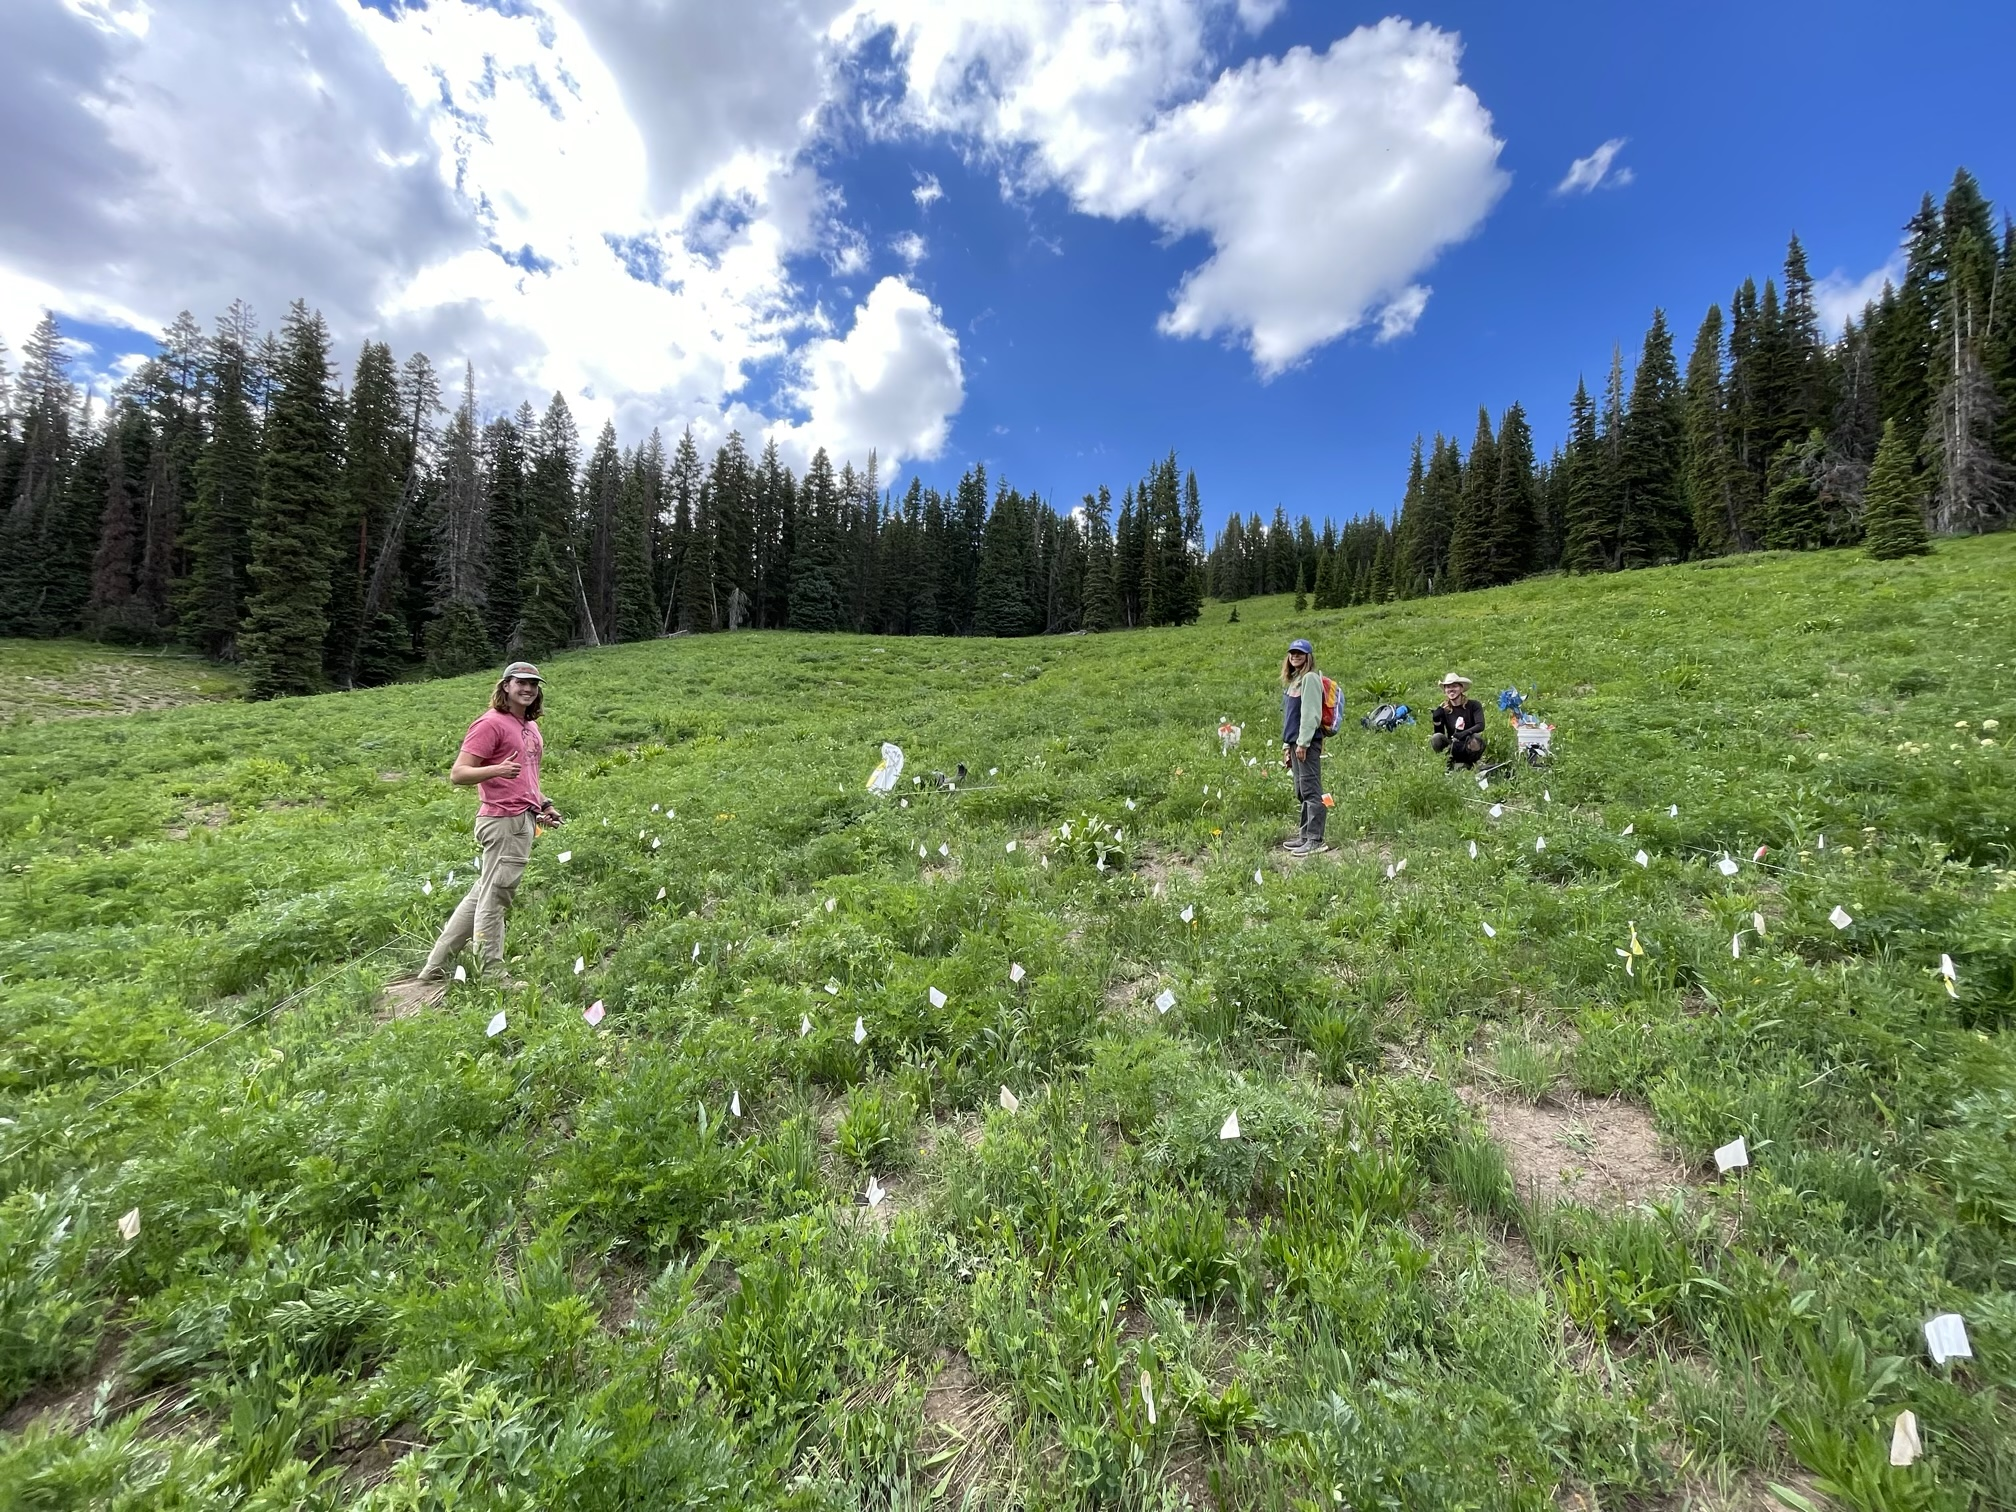
\includegraphics[width=6in,height=\textheight,keepaspectratio]{../static/clipping-experiment.jpg}

}

\caption{Clipping flower buds to manipulate the density and species
composition around focal plants in Colorado. (L to R): Ben Davis, Sarah
Hoffman, Alden Sears.}

\end{figure}%

\subsection{Selected publications}\label{selected-publications}

\begin{itemize}
\item
  Petry, W.K., Kandlikar, G.S., Kraft, N.J.B., Godoy, O. \& Levine, J.M.
  \textbf{(2018)} A competition-defence trade-off both promotes and
  weakens coexistence in an annual plant community. \ul{\emph{Journal of
  Ecology}}, 106, 1806--1818.
  \href{https://doi.org/10.1111/1365-2745.13028}{{[}doi{]}}
  \href{publications/Petry\%20et\%20al.\%20-\%202018\%20-\%20A\%20competition–defence\%20trade-off\%20both\%20promotes\%20and\%20.pdf}{{[}pdf{]}}
  \href{https://doi.org/10.5281/zenodo.1256658}{{[}data{]}}
\item
  Blonder, B.W., Gaüzère, P., Iversen, L.L., Ke, P.-J., Petry, W.K.,
  Ray, C.A., Salguero-Gómez, R., Sharpless, W., Violle, C.
  \textbf{(2023)} Predicting and controlling ecological communities via
  trait and environment mediated parameterizations of dynamical models.
  \ul{\emph{Oikos}}, 2023, e09415.
  \href{https://doi.org/10.1111/oik.09415}{{[}doi{]}}
  \href{publications/Blonder\%20et\%20al.\%20-\%202023\%20-\%20Predicting\%20and\%20controlling\%20ecological\%20communities\%20via\%20trait\%20and\%20environment\%20mediated\%20parameterizatio.pdf}{{[}pdf{]}}
  \href{https://zenodo.org/record/7576397}{{[}data{]}}
\item
  Petry, W.K., Perry, K.I., Fremgen, A., Rudeen, S.K., Lopez, M.,
  Dryburgh, J., Mooney, K.A. \textbf{(2013)} Mechanisms underlying plant
  sexual dimorphism in multi-trophic arthropod communities.
  \ul{\emph{Ecology}}, 94, 2055--2065.
  \href{https://doi.org/10.1890/12-2170.1}{{[}doi{]}}
  \href{publications/Petry\%20et\%20al.\%20-\%202013\%20-\%20Mechanisms\%20underlying\%20plant\%20sexual\%20dimorphism\%20in\%20m.pdf}{{[}pdf{]}}
\end{itemize}




\end{document}
